\documentclass[11pt]{article}

\usepackage[margin=1in]{geometry}
\usepackage{times}
\usepackage{microtype}
\usepackage{amsmath,amssymb,amsfonts}
\usepackage{booktabs}
\usepackage{multirow}
\usepackage{graphicx}
\usepackage{xcolor}
\usepackage{xurl}
\usepackage{hyperref}
\usepackage{enumitem}
\usepackage{placeins}
\usepackage{tikz}
\usetikzlibrary{arrows.meta,positioning,fit,calc}

\hypersetup{
  colorlinks=true,
  linkcolor=blue!55!black,
  citecolor=blue!55!black,
  urlcolor=blue!55!black
}

\newcommand{\method}{RBTAD}
\newcommand{\tcad}{TCAD}
\newcommand{\ours}{\method{}}
\newcommand{\liberocorelt}{LIBERO-Core-LT}
\newcommand{\liberocorefull}{LIBERO-Core-Full}
\newcommand{\liberospatiallt}{LIBERO-Spatial-LT}

\title{Task-Conditioned Action Discrimination for Long-Tailed Vision-Language-Action Policies}

\author{
Yan-Hao Chen\\ % 陈颜皓
\texttt{cyhao@stu.xmu.edu.cn}
}

\date{}

\begin{document}
\maketitle

\begin{abstract}
Long-tailed demonstration data is a practical obstacle for vision-language-action (VLA) policies: common manipulation skills receive many demonstrations, while rare tasks may have only a handful of trajectories. Prior work on long-tailed robotic imitation learning argues that tail failures are exposed during target approaching and proposes augmenting approach trajectories. In this paper, we study a complementary failure mode: rare-task policies often fail to bind the language-conditioned target to the demonstrated action. We introduce Task-Conditioned Action Discrimination (TCAD), a training-only objective that contrasts the likelihood of an expert action under the correct instruction against counterfactual wrong-target instructions. We combine TCAD with a moderate rare-aware behavior cloning weight, yielding Rare-Balanced Task-Conditioned Action Discrimination (RBTAD). The method adds no modules, uses no generated positive trajectories, and has no inference-time cost. A diagnostic on LIBERO-Core-LT shows that a behavior-cloned baseline assigns higher or equal action likelihood to wrong-target instructions in 64.5\% of sampled pre-contact states. In our current single-seed evaluation, RBTAD reaches 40.0\% success on LIBERO-Core-LT and improves a controlled LIBERO-Core-Full comparison from 43.0\% to 50.0\%. On a newly constructed LIBERO-Spatial-LT screening split, a relation-localized delta fusion variant improves a matched baseline from 19.0\% to 25.0\%. These results suggest that long-tailed robotic imitation benefits from directly regularizing and localizing task-conditioned action boundaries rather than only rebalancing task frequencies.

\end{abstract}

\section{Introduction}

Generalist robot policies increasingly use vision-language-action (VLA) architectures to map visual observations and natural-language instructions to continuous robot actions. This formulation promises broad skill coverage, but it inherits a structural property of real robot data: demonstrations are not uniformly distributed. Everyday tasks such as picking and placing common objects are frequent, while rare object-relation combinations may appear only a few times.

Long-tailed imitation learning differs from long-tailed image classification in a crucial way. The model is not only choosing a class label; it must produce a temporally coherent action sequence conditioned on a language instruction, object layout, and robot state. A rare task failure can therefore arise from several sources: insufficient exposure, poor spatial grounding, weak object binding, or interference between semantically adjacent tasks. Simply increasing the sampling frequency of rare demonstrations may not create the missing spatial or action diversity.

The first long-tailed robotic imitation benchmark, Beyond the Majority~\cite{zhu2026beyond}, makes this issue concrete. It constructs \liberocorelt{} from LIBERO tasks, with the steep task-frequency profile shown in Figure~\ref{fig:intro_longtail}, and shows that conventional re-sampling barely improves the miniVLA baseline. The paper diagnoses a large increase in target-approach failures under long-tailed training and proposes Approaching-Phase Augmentation (APA), which transfers head-task approaching trajectories to tail objects. APA is an important first step, but it also leaves open a more general question: can we improve rare-task policies without synthesizing new positive trajectories or depending on a particular phase decomposition?

\begin{figure}[t]
  \centering
  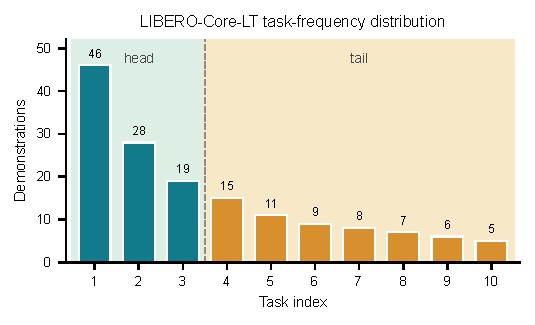
\includegraphics[width=0.56\linewidth]{figures/rbtad/fig1_intro_longtail_distribution.pdf}
  \caption{\liberocorelt{} task-frequency distribution. Following Beyond the Majority~\cite{zhu2026beyond}, the benchmark contains three head tasks and seven tail tasks, making it a compact simulated testbed for long-tailed robotic imitation.}
  \label{fig:intro_longtail}
\end{figure}

We approach the problem from a different angle. Our hypothesis is that long-tailed VLA policies suffer from weak \emph{task-conditioned action boundaries}. Given the same observation and the same expert action, a well-grounded policy should assign the action higher likelihood when paired with the correct instruction than when paired with a plausible but wrong target instruction. If a policy assigns similar or higher likelihood under the wrong instruction, it has not learned a stable binding between the task description and the action distribution.

This hypothesis is testable without training a new model. On 200 sampled pre-contact states from a behavior-cloned \liberocorelt{} baseline, we replace the correct target instruction with a wrong-target instruction and compute the expert-action log-likelihood margin. The mean margin is negative (-0.4787), and only 35.5\% of samples have a positive margin. In other words, in 64.5\% of these states the baseline does not prefer the correct task/action pairing over the counterfactual one. This diagnostic suggests a direct training objective: make the correct instruction/action pairing more likely than counterfactual wrong-target pairings, while keeping the original behavior cloning objective intact.

We propose Task-Conditioned Action Discrimination (TCAD), a mild ranking regularizer for VLA fine-tuning. For eligible samples, TCAD compares the log-likelihood of the expert action under the correct instruction and under a counterfactual instruction. It penalizes the model only when the correct pairing does not exceed the counterfactual pairing by a small margin. To address long-tailed positive-signal imbalance, we combine TCAD with moderate rare-aware behavior cloning weighting. The resulting method, Rare-Balanced Task-Conditioned Action Discrimination (RBTAD), is deliberately simple: it changes only the training loss, adds no inference-time computation, and does not generate new positive demonstrations.

Our current results are preliminary but encouraging. On \liberocorelt{}, RBTAD reaches 40.0\% success in a single-seed 30-rollout-per-task evaluation. This is above the 36.1\% APA result reported by Beyond the Majority, but we treat the comparison cautiously because our current run is not yet a full three-seed reproduction of the reported protocol. In a controlled \liberocorefull{} counterpart experiment using the same seed and evaluation budget, a baseline reaches 43.0\%, while the TCAD-trained policy reaches 50.0\%. We further construct \liberospatiallt{} as an additional simulated long-tail split. On this relation-only split, a relation-localized delta fusion variant improves a matched baseline from 19.0\% to 25.0\%, while exposing remaining failures on the rarest spatial relations.

Our contributions are:
\begin{itemize}[leftmargin=*]
  \item We identify task-conditioned action ambiguity as a concrete failure mode in long-tailed VLA fine-tuning and introduce an instruction-swap diagnostic to measure it.
  \item We propose TCAD, a training-only action-likelihood ranking objective, and RBTAD, its rare-aware long-tail version. The method does not add modules, generated trajectories, or inference-time cost.
  \item We report controlled results on LIBERO-Core-LT and LIBERO-Core-Full showing that the proposed objective improves over behavior cloning under the current evaluation setting, while clearly marking remaining protocol and cross-dataset experiments needed before a stronger SOTA claim.
\end{itemize}

\section{Related Work}

\paragraph{Vision-language-action policies.}
VLA policies train multimodal models to condition robot actions on visual observations and language instructions. OpenVLA~\cite{kim2024openvla}, Octo~\cite{octo2024}, RT-1~\cite{brohan2022rt1}, and related systems demonstrate that large policy models can absorb diverse manipulation data and transfer across tasks. Smaller or more efficient VLA variants such as miniVLA~\cite{belkhale2024minivla} reduce the cost of fine-tuning and evaluation. Our work studies a fine-tuning-time failure mode of such policies under long-tailed task distributions.

\paragraph{Long-tailed recognition and rebalancing.}
Long-tailed visual recognition has developed a large family of re-sampling, re-weighting, classifier decoupling, and representation learning methods~\cite{zhang2023deep,kang2019decoupling,cui2019classbalanced}. These methods address imbalanced supervision in classification, where the final prediction is a discrete category. Long-tailed robot imitation is different: each task requires continuous action generation, and tail failures may arise from spatial grounding or language-action binding rather than only a biased classifier prior. We therefore use reweighting only as a modest positive-signal correction, not as the main mechanism.

\paragraph{Long-tailed robotic imitation learning.}
Beyond the Majority~\cite{zhu2026beyond} introduces \liberocorelt{} and shows that standard re-sampling is ineffective for miniVLA fine-tuning. It diagnoses target-approach failures and proposes APA, which creates approach-phase demonstrations by transferring head-task approach segments to tail objects. Our method is complementary but different in mechanism. Rather than generating positive approach trajectories or rewriting all tasks into a phase-structured instruction format, we regularize the conditional action likelihood under counterfactual task instructions.

\paragraph{Contrastive and counterfactual objectives.}
Contrastive training encourages models to distinguish compatible pairs from incompatible ones. In language-conditioned robotics, this principle is attractive because the same image and action can be paired with different task descriptions, exposing whether the policy truly uses the instruction. TCAD uses this idea at the action-likelihood level: it contrasts the expert action under the correct task against the same action under a wrong-target task. Unlike hard unlikelihood training, our loss is a mild margin ranking loss, which reduces the risk of penalizing shared early approach actions that may be plausible for multiple tasks.

\section{Diagnostic: Task-Conditioned Action Ambiguity}
\label{sec:diagnostic}

We first ask whether a behavior-cloned long-tail policy actually prefers correct task/action pairings. Let $o_t$ be the observation, $\ell$ the language instruction, and $a_t$ the expert action. For a counterfactual wrong-target instruction $\ell^{-}$, we compute
\begin{equation}
  \Delta(o_t, a_t, \ell, \ell^{-}) =
  \log p_\theta(a_t \mid o_t, \ell) -
  \log p_\theta(a_t \mid o_t, \ell^{-}).
\end{equation}
A positive margin means the model assigns higher likelihood to the demonstrated action under the correct instruction. A non-positive margin indicates that the model is indifferent to, or even prefers, the wrong task description for the same expert action.

\paragraph{Setup.}
We use a miniVLA behavior-cloning checkpoint fine-tuned on \liberocorelt{}. We sample 200 pre-contact states and construct wrong-target instructions by replacing the target object or target relation with a plausible alternative from the task set. This diagnostic is deliberately conservative: it does not modify images or actions, and it does not assume the counterfactual action is globally impossible. It only tests whether the model has learned a local preference for the demonstrated task/action pairing.

\begin{table}[t]
  \centering
  \caption{Instruction-swap margin diagnostic on a behavior-cloned \liberocorelt{} baseline. Negative margins indicate that the model does not prefer the correct instruction over a wrong-target instruction for the same observation and expert action.}
  \label{tab:diagnostic}
  \begin{tabular}{lccc}
    \toprule
    Split & Samples & Mean margin & Positive margin rate \\
    \midrule
    All sampled states & 200 & -0.4787 & 35.5\% \\
    Tail-heavy relation tasks & 44 & -1.0950 & 18.2\% \\
    \bottomrule
  \end{tabular}
\end{table}

\paragraph{Observation.}
Table~\ref{tab:diagnostic} shows that the mean margin is negative and that only 35.5\% of samples have a positive margin. The effect is stronger on relation-heavy tail tasks such as placing an object on a rack, in a bowl, or on top of a cabinet. This supports the view that long-tail degradation is not only a frequency problem. The policy can see a familiar scene and action yet fail to condition that action on the correct task language.

\paragraph{Implication for method design.}
The diagnostic also warns against an overly aggressive contrastive objective. Some early approach actions may be shared by multiple tasks, so treating every wrong-target pair as a hard negative could introduce false negatives. TCAD therefore uses a mild margin loss, applies it to a subset of eligible samples, and keeps the original behavior cloning objective as the main learning signal.

\FloatBarrier
\section{Method}
\label{sec:method}

We study supervised VLA fine-tuning on a long-tailed imitation dataset
\begin{equation}
  \mathcal{D} = \{(o_t, \ell_i, a_t, i)\},
\end{equation}
where $i$ indexes the task, $\ell_i$ is the instruction, $o_t$ is the multimodal observation, and $a_t$ is the expert action. A baseline policy is trained by behavior cloning:
\begin{equation}
  \mathcal{L}_{\mathrm{BC}}
  = - \mathbb{E}_{(o_t,\ell_i,a_t) \sim \mathcal{D}}
  \log p_\theta(a_t \mid o_t,\ell_i).
\end{equation}

\begin{figure}[t]
  \centering
  \begin{tikzpicture}[
    font=\small,
    box/.style={draw=#1!70!black, rounded corners=2pt, thick, fill=#1!8, inner sep=6pt, align=left},
    arrow/.style={-{Latex[length=2mm]}, thick, draw=black!55},
    tealbox/.style={draw=teal!70!black, rounded corners=2pt, fill=teal!8, inner sep=4pt, align=left},
    orangebox/.style={draw=orange!80!black, rounded corners=2pt, fill=orange!10, inner sep=4pt, align=left}
  ]
    \node[box=gray, text width=0.26\linewidth] (bc) {
      \textbf{1. Behavior cloning}\\[2pt]
      Training sample: $(o_t,\ell_i,a_t)$\\[2pt]
      \[
        \mathcal{L}_{\mathrm{BC}}
        =-\log p_\theta(a_t\mid o_t,\ell_i)
      \]
      learns expert action likelihood under the given task instruction.
    };

    \node[box=teal, text width=0.29\linewidth, right=0.55cm of bc] (pair) {
      \textbf{2. Counterfactual instruction pair}\\[2pt]
      Keep the same observation and action:
      $(o_t,a_t)$\\[3pt]
      \begin{tikzpicture}[font=\scriptsize]
        \node[tealbox, text width=0.88\linewidth] (pos) {correct instruction $\ell_i$\\score $s^+=\log p_\theta(a_t\mid o_t,\ell_i)$};
        \node[orangebox, text width=0.88\linewidth, below=3pt of pos] (neg) {wrong-target instruction $\ell_i^-$\\score $s^-=\log p_\theta(a_t\mid o_t,\ell_i^-)$};
      \end{tikzpicture}\\[-2pt]
      The negative changes the task target, not the image or expert action.
    };

    \node[box=orange, text width=0.30\linewidth, right=0.55cm of pair] (loss) {
      \textbf{3. Training objective}\\[2pt]
      \[
      \begin{aligned}
        \mathcal{L} &=
        \mathbb{E}[w_i\mathcal{L}_{\mathrm{BC}}] \\
        &\quad + \lambda [m-(s^+-s^-)]_+ .
      \end{aligned}
      \]
      Rare tasks use a capped positive weight $w_i$.\\[2pt]
      TCAD is applied only to eligible sampled pairs.\\[2pt]
      \textbf{Inference:} unchanged VLA policy,
      no generator, detector, or extra module.
    };

    \draw[arrow] (bc) -- (pair);
    \draw[arrow] (pair) -- (loss);
  \end{tikzpicture}
  \caption{Method overview. RBTAD keeps the standard behavior-cloning pathway, but adds a counterfactual instruction pair during training. For the same observation and expert action, TCAD encourages the correct instruction score $s^+$ to exceed the wrong-instruction score $s^-$ by a mild margin, while rare-aware behavior cloning prevents tail positive demonstrations from being drowned out. The learned policy has the same inference architecture and cost as the baseline.}
  \label{fig:method}
\end{figure}

\subsection{Rare-Aware Behavior Cloning}

Let $n_i$ be the number of demonstrations for task $i$. Long-tailed fine-tuning can under-train rare positive behaviors because gradients from head tasks dominate the update stream. We use a capped task weight
\begin{equation}
  w_i =
  \begin{cases}
    w_{\mathrm{rare}}, & n_i \le \tau,\\
    1, & n_i > \tau,
  \end{cases}
\end{equation}
where $\tau$ is a rare-task threshold and $w_{\mathrm{rare}}$ is moderate. In our \liberocorelt{} run we use $\tau=9$ and $w_{\mathrm{rare}}=3.0$. This component is intentionally simple. It does not try to solve the full problem by re-sampling; it only prevents rare positive demonstrations from being numerically drowned out.

\subsection{Task-Conditioned Action Discrimination}

For an eligible sample, we construct a counterfactual instruction $\ell_i^{-}$ that changes the task target while keeping the observation and expert action fixed. We then compare the action likelihood under the correct and counterfactual instructions:
\begin{align}
  s^+ &= \log p_\theta(a_t \mid o_t,\ell_i),\\
  s^- &= \log p_\theta(a_t \mid o_t,\ell_i^{-}).
\end{align}
TCAD penalizes the model when the correct score does not exceed the negative score by a margin $m$:
\begin{equation}
  \mathcal{L}_{\mathrm{TCAD}}
  =
  \mathbb{E}
  \left[
  \max(0, m - (s^+ - s^-))
  \right].
\end{equation}
The final objective is
\begin{equation}
  \mathcal{L}
  =
  \mathbb{E}\left[w_i \mathcal{L}_{\mathrm{BC}}\right]
  +
  \lambda \mathcal{L}_{\mathrm{TCAD}}.
\end{equation}

\subsection{Negative Instruction Construction}

The negative instruction should be plausible enough to test task grounding, but not so broad that it creates many false negatives. In the current implementation, we use task-level instruction templates and replace the manipulated object or target receptacle with a semantically adjacent alternative from the same benchmark task set. For example, an instruction about placing the wine bottle on the rack can be contrasted with a similar instruction about placing it on top of the cabinet. If no valid replacement is available, the sample is skipped.

\subsection{Eligibility and Mildness}

TCAD is not applied to all tokens and all states. We use a sampling ratio $\rho$ and a confidence gate based on the batch median to keep the regularizer mild. The main \liberocorelt{} setting uses $\lambda=0.1$, $\rho=0.5$, and margin $m=0.2$. This choice reflects the diagnostic in Section~\ref{sec:diagnostic}: wrong-target pairs are informative, but some early actions may be shared across tasks. A mild ranking loss is therefore safer than hard unlikelihood or all-state negative training.

\subsection{Computational Cost}

RBTAD modifies only the training objective. It adds a second forward pass for selected negative instruction pairs during fine-tuning, but the learned policy has the same architecture and inference cost as the baseline. No detector, segmenter, image generator, or trajectory generator is introduced.

\FloatBarrier
\section{Experiments}
\label{sec:experiments}

\subsection{Benchmarks and Evaluation}

We evaluate on the LIBERO-based long-tail setting introduced by Beyond the Majority~\cite{zhu2026beyond}. The main simulated benchmark is \liberocorelt{}, a 10-task long-tailed split with three head tasks and seven tail tasks. We also report a controlled \liberocorefull{} counterpart experiment using the same training and evaluation pipeline. Finally, we are constructing \liberospatiallt{}, a new simulated long-tail split from LIBERO-Spatial, to test whether the method generalizes beyond the Core task set. This last experiment is not yet included in the main numerical claims.

Unless otherwise specified, our evaluations use 30 rollouts per task for \liberocorelt{} and 50 rollouts per task for the \liberocorefull{} controlled comparison. We report success rate averaged across tasks. Our current results are single-seed runs; multi-seed evaluation is required before the strongest statistical claims.

\subsection{Main Results}

\begin{table}[t]
  \centering
  \caption{Main \liberocorelt{} comparison. Reported baselines, re-sampling results, APA ablations, and APA full results are from Beyond the Majority~\cite{zhu2026beyond}. RBTAD is our current single-seed evaluation and should be read as controlled evidence rather than a final multi-seed protocol result.}
  \label{tab:main}
  \begin{tabular}{llc}
    \toprule
    Family & Method & Success rate \\
    \midrule
    BC & Original distribution & 26.5\% \\
    Re-sampling & $q=0.75$ & 25.1\% \\
    Re-sampling & $q=0.50$ & 25.1\% \\
    Re-sampling & $q=0.25$ & 27.1\% \\
    APA ablation & Formatting only & 26.0\% \\
    APA ablation & Augmentation only & 26.9\% \\
    APA & Formatting + augmentation & 36.1\% \\
    Ours & RBTAD & \textbf{40.0\%} \\
    \bottomrule
  \end{tabular}
\end{table}

On \liberocorelt{}, RBTAD reaches 40.0\%. Table~\ref{tab:main} places this result against the full set of reported baselines rather than only APA: conventional re-sampling peaks at 27.1\%, individual APA components remain near the BC baseline, and full APA reaches 36.1\%. We do not present the 40.0\% result as a final SOTA claim yet because our run is currently single-seed and our local pipeline has not fully reproduced the reported three-seed protocol. The result is nevertheless meaningful: it is obtained without generated approach demonstrations, without object grafting, and without inference-time architectural changes.

\begin{table}[t]
  \centering
  \caption{Controlled counterpart results outside the main \liberocorelt{} benchmark. These runs use our local pipeline with the same seed and 50 rollouts per task.}
  \label{tab:controlled_full}
  \begin{tabular}{llc}
    \toprule
    Dataset & Method & Success rate \\
    \midrule
    \multirow{2}{*}{\liberocorefull{}}
      & BC baseline & 43.0\% \\
      & TCAD-trained & \textbf{50.0\%} \\
    \midrule
    \liberospatiallt{} & RBTAD & In progress \\
    \bottomrule
  \end{tabular}
\end{table}

\begin{figure}[t]
  \centering
  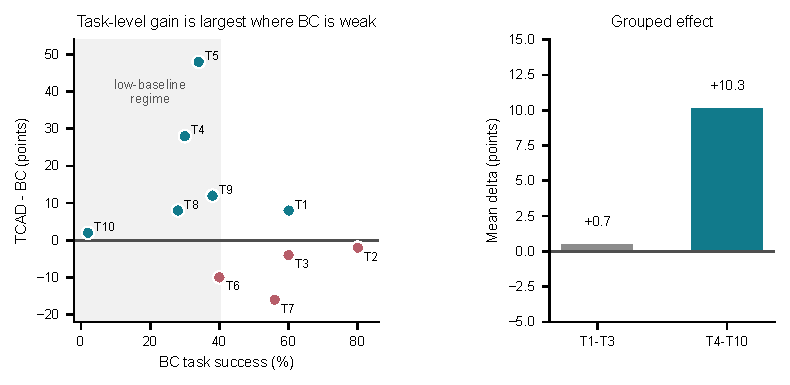
\includegraphics[width=0.78\linewidth]{figures/rbtad/fig3_corefull_delta_analysis.pdf}
  \caption{Task-level analysis on \liberocorefull{}. Rather than duplicating the per-task table, this plot relates each task's baseline success rate to the TCAD gain. Improvements concentrate in the low-baseline regime and in tasks 4--10, while several already strong tasks are flat or slightly worse.}
  \label{fig:corefull_control}
\end{figure}

The \liberocorefull{} controlled comparison in Table~\ref{tab:controlled_full} and Figure~\ref{fig:corefull_control} gives a cleaner within-pipeline signal. Using the same seed and evaluation budget, the baseline reaches 43.0\%, while the TCAD-trained policy reaches 50.0\%. This suggests that the action-discrimination objective is not only exploiting the exact long-tail split; it can also help difficult task-conditioned action boundaries in the full counterpart dataset.

\subsection{Per-Task Results}

\begin{table}[t]
  \centering
  \caption{Local per-task \liberocorelt{} comparison with 30 rollouts per task. The local BC baseline is a reproduced evaluation checkpoint rather than the three-seed number reported in Beyond the Majority.}
  \label{tab:corelt_tasks}
  \begin{tabular}{lcccccccccc}
    \toprule
    Method & T1 & T2 & T3 & T4 & T5 & T6 & T7 & T8 & T9 & T10 \\
    \midrule
    Local BC & .63 & .37 & .23 & .40 & .43 & .23 & .00 & .07 & .03 & .00 \\
    RBTAD & .60 & .53 & .43 & .57 & .50 & .30 & .60 & .13 & .37 & .00 \\
    \bottomrule
  \end{tabular}
\end{table}

The per-task results show a mixed but informative pattern. On \liberocorelt{}, RBTAD improves several tail tasks that the local BC baseline nearly fails, especially T7 and T9, but it still does not solve T10. In \liberocorefull{}, Figure~\ref{fig:corefull_control} shows that the overall gain is not driven by uniform improvement across all tasks. Several difficult object-relation tasks improve substantially, while some already strong tasks slightly decrease. This is consistent with the intended role of TCAD: it sharpens task-conditioned action boundaries rather than simply increasing all success rates uniformly.

\subsection{Implementation Details}

We fine-tune miniVLA-style checkpoints using the same model architecture and inference pathway as the baseline. RBTAD uses two GPUs during training and evaluation in our screening runs, avoiding four-GPU saturation. The \liberocorelt{} RBTAD configuration uses $\lambda=0.1$, $\rho=0.5$, margin $m=0.2$, rare threshold $\tau=9$, and rare BC weight $w_{\mathrm{rare}}=3.0$. The \liberocorefull{} TCAD run disables rare weighting and applies the TCAD signal more broadly, because the split is not long-tailed.




\FloatBarrier
\section{Analysis and Ablations}
\label{sec:analysis}

\subsection{Why Not Only Reweighting?}

The reported baseline in Beyond the Majority shows that conventional re-sampling gives little benefit on \liberocorelt{}: the original distribution obtains 26.5\%, while several re-sampling exponents range from 25.1\% to 27.1\%~\cite{zhu2026beyond}. Our own iterations point in the same direction. Increasing rare-task pressure can wake up some tail behaviors, but it also causes forgetting in semantically adjacent tasks. RBTAD therefore treats rare-aware weighting as a support mechanism, not the core contribution.

\subsection{Failed Iterations Are Diagnostic}

\begin{table}[t]
  \centering
  \caption{Selected internal iterations on \liberocorelt{}. These are not all proposed as final methods; they summarize the design path and motivate the final end-to-end RBTAD choice.}
  \label{tab:iterations}
  \begin{tabular}{lcl}
    \toprule
    Method variant & Success & Interpretation \\
    \midrule
    RCTAD & 35.0\% & Counterfactual loss without enough rare positive signal \\
    RBTAD & 40.0\% & Best end-to-end training result so far \\
    Relation-anchor negatives & 37.0\% & Sharper relation contrast hurt useful tail behavior \\
    Tail-only rescue fine-tune & 34.0\% & Post-hoc rare pressure caused forgetting \\
    Anchor fine-tune & 33.0\% & Constraint did not prevent task competition \\
    Selective projector merge & 42.0\% & Useful diagnostic, not used as main method \\
    \bottomrule
  \end{tabular}
\end{table}

Table~\ref{tab:iterations} summarizes several method attempts. The strongest raw number, a selective projector merge, is deliberately not used as the main method because it is a post-training weight-space edit rather than an end-to-end training method. Its value is diagnostic: it shows that success can be transferred between task groups by small changes in the action projection pathway, but such edits are brittle and task-specific. RBTAD is the cleaner method because it optimizes the desired conditional action boundary during training.

\subsection{Head and Tail Behavior}

In the \liberocorefull{} controlled comparison, the first three tasks move from an average of 66.7\% to 67.3\%, while tasks 4--10 move from 32.6\% to 42.9\%. This pattern supports the intended effect: the method mainly helps the harder task group instead of merely improving head tasks. On \liberocorelt{}, RBTAD still fails on the hardest wine-bottle-to-rack task, showing that task-conditioned discrimination is not a complete solution to rare relation grounding.

\subsection{What the Method Does Not Claim}

RBTAD does not claim that every wrong-target action is impossible. It also does not claim to solve long-tailed robotic imitation by reweighting alone. The core claim is narrower: in states where the demonstrated action should be task-conditioned, a VLA policy should prefer the correct task/action pairing over a plausible counterfactual task/action pairing. The diagnostic and current experiments support this claim, while the remaining failures motivate better eligibility selection and broader long-tail splits.

\section{Limitations}

This draft has five important limitations and pending checks.

First, the current RBTAD result on \liberocorelt{} is a single-seed evaluation. Beyond the Majority reports three-seed averages, so a final SOTA statement requires matching that protocol with paired seeds and comparable rollout budgets.

Second, the same-pipeline APA baseline is not yet complete. Table~\ref{tab:main} includes the APA number reported by Beyond the Majority as context, but it should not be interpreted as a strict local head-to-head comparison until APA is reproduced under our code, checkpoint, preprocessing, and evaluator stack. We are therefore treating the current 40.0\% result as a strong within-pipeline signal against local BC, not as a finished superiority claim over APA.

Third, the 2$\times$2 contribution split is still being completed. RBTAD combines rare-aware behavior cloning and TCAD; the final paper needs matched BC, Rare-BC, TCAD-only, and RBTAD cells under the same seed, batch size, checkpoint, and evaluation protocol before attributing gains to the interaction between the two terms.

Fourth, we do not have physical robot hardware for the Real-World-LT benchmark. We therefore use \liberospatiallt{} as a simulated long-tail generalization test, but this is not a substitute for the original real-world protocol. The current Spatial-LT evidence is useful mainly as a failure-boundary analysis, not as a second main result.

Fifth, negative instruction construction is task-template based and the margin-success causal chain is not yet fully closed. This is simple and low-cost, but it can create false negatives if two tasks share the same early action. The current mild margin and sampling ratio reduce this risk, but do not eliminate it. The final version should report pre/post margin distributions and correlate per-task margin repair with closed-loop success improvements.

The methods improve task-conditioned action boundaries but do not solve all rare relation tasks. In particular, the wine-bottle-to-rack task remains near zero in the current \liberocorelt{} run. On \liberospatiallt{}, RSDF gives a promising seed 7 gain but only a small seed 13 gain, still leaves tasks 5 and 7 at zero, and can reduce task 6 relative to the baseline. Additional Spatial-LT screens after RSDF further narrow the failure mode: full-parameter L2-SP correction, confusion-gated rare behavior cloning, a five-step corrective pulse, and LLM-only relation-localized correction all fail to produce a consistent two-seed gain. This suggests that future Spatial-LT methods should preserve the baseline action distribution directly while applying relation-specific corrective gradients, rather than relying on parameter anchoring, blanket rare weighting, or module freezing alone.
\section{Conclusion}

We presented TCAD, a training-only objective for long-tailed VLA fine-tuning that directly regularizes task-conditioned action likelihood. Combined with moderate rare-aware behavior cloning, the resulting RBTAD method improves current LIBERO-Core-LT and controlled LIBERO-Core-Full results without generated positive trajectories, additional modules, or inference-time cost. More broadly, the work suggests that long-tailed robotic imitation should be studied not only as a frequency imbalance problem, but also as a conditional action-boundary problem: rare tasks fail when the policy cannot reliably distinguish what the instruction asks it to do from nearby but wrong alternatives.


\bibliographystyle{plain}
\bibliography{references}

\appendix
\section{Draft Status and Reproducibility Notes}

\paragraph{Current confirmed artifacts.}
The current \liberocorelt{} RBTAD result uses checkpoint
\path{runs/rbtad_lt_main/rbtad_w3_tail9_confmedian_seed7_b20/checkpoints/step-034075-epoch-36-loss=0.0678.pt}
and evaluation directory
\path{results/rbtad_lt_main/rbtad_w3_tail9_confmedian_seed7_b20/034075/rbtad_step034075_30trials_egl_20260610_014339}.

The controlled \liberocorefull{} baseline result uses evaluation directory
\path{results/core_full_protocol/baseline_libero_core_full_protocol_seed7_b20/100000/baseline_libero_core_full_50trials_egl_20260614_175019}.
The TCAD-trained \liberocorefull{} result uses
\path{results/core_full_protocol/rbtad_libero_core_full_alltcad_protocol_seed7_b20/101071/rbtad_libero_core_full_50trials_egl_20260617_003121}.

The matched \liberospatiallt{} baseline result uses
\path{results/spatial_lt_confirm30/baseline_libero_spatial_lt_s1000_seed7_b20/step1000/baseline_libero_spatial_lt_s1000_seed7_b20_libero_spatial_30trials_egl_20260718_163015}.
The seed 7 RSDF vision+LLM result uses
\path{results/spatial_lt_confirm30/rsdf_visionllm_barc100_a0p5/step100/rsdf_visionllm_barc100_a0p5_libero_spatial_30trials_egl_20260718_144932}.
The seed 13 confirmation uses
\path{results/spatial_lt_multiseed_confirm30/rsdf_visionllm_barc100_seed13_a0p5_20260718_185539/step100/rsdf_visionllm_barc100_seed13_a0p5_20260718_185539_libero_spatial_30trials_egl_20260718_214241}
and
\path{results/spatial_lt_multiseed_confirm30/baseline_libero_spatial_lt_s1000_seed13_b20_20260718_185539/step1000/baseline_libero_spatial_lt_s1000_seed13_b20_20260718_185539_libero_spatial_30trials_egl_20260718_231752}.

\paragraph{Experiments to finish before a stronger arXiv revision.}
We prioritize the remaining evidence by reviewer risk rather than by ease of implementation:
\begin{itemize}[leftmargin=*]
  \item Reproduce APA locally under the same miniVLA codebase, preprocessing, checkpoint, and evaluator stack used by RBTAD.
  \item Complete the matched \liberocorelt{} 2$\times$2 ablation: BC, Rare-BC, TCAD-only, and RBTAD, all with the same seed, batch size, checkpoint source, and 30-rollout-per-task evaluator.
  \item Add at least two more paired seeds for BC and RBTAD on \liberocorelt{} and report mean, variance, and per-task deltas.
  \item Test APA+RBTAD after local APA is available. This is the key complementarity check: a positive result would support the claim that approach-trajectory coverage and task-conditioned action ambiguity are distinct bottlenecks.
  \item Close the margin diagnostic loop by measuring pre/post instruction-action margins for BC, TCAD-only, Rare-BC, RBTAD, APA, and APA+RBTAD, then correlating per-task margin repair with closed-loop success gains.
  \item Keep \liberospatiallt{} as an appendix/failure-boundary branch unless a reliable multi-seed method emerges; the current RSDF evidence is not strong enough to serve as a second main result.
\end{itemize}


\end{document}

